\section{The basics of regression and classification}

\newcommand{\weightnode}[3]{
    \node[circle, draw=black, fill=teal!60, opacity=#3] at (#1, #2*3.5) {};
}

\newcommand{\weightplot}[1]{
    \begin{tikzpicture}
        \ifnum#1<3
            \draw[|-Latex] (0, 3.3*3.5) -- (0, 4.6*3.5);
            \weightnode{0}{3.850}{1.0}
            \weightnode{0}{4.354}{1.0}
        \fi
        \ifnum#1>2
            \draw[|-Latex,black!20] (0, 3.3*3.5) -- (0, 4.6*3.5);
            \weightnode{0}{3.850}{0.2}
            \weightnode{0}{4.354}{0.2}
        \fi
        \ifnum#1=1
            \weightnode{0}{3.504}{1.0}
            \weightnode{0}{3.693}{1.0}
            \weightnode{0}{3.436}{1.0}
            \weightnode{0}{3.433}{1.0}
            \weightnode{0}{3.449}{1.0}
            \weightnode{0}{4.341}{1.0}
            \weightnode{0}{4.354}{1.0}
            \weightnode{0}{4.312}{1.0}
            \weightnode{0}{4.425}{1.0}
        \fi
        \ifnum#1>1
            \weightnode{0}{3.504}{0.2}
            \weightnode{0}{3.693}{0.2}
            \weightnode{0}{3.436}{0.2}
            \weightnode{0}{3.433}{0.2}
            \weightnode{0}{3.449}{0.2}
            \weightnode{0}{4.341}{0.2}
            \weightnode{0}{4.354}{0.2}
            \weightnode{0}{4.312}{0.2}
            \weightnode{0}{4.425}{0.2}

            \ifnum#1=2
                \draw[|-|, dashed] (0.5, 3.850*3.5) -- (0.5, 4.354*3.5);
                \node[anchor=west] at (0.5, 4.102*3.5) {\small{504}};
            \fi
        \fi
    \end{tikzpicture}
}

\newsavebox{\weightboxfirst}
\sbox{\weightboxfirst}{
    \weightplot{1}
}

\newsavebox{\weightboxsecond}
\sbox{\weightboxsecond}{
    \weightplot{2}
}

\newsavebox{\weightboxhidden}
\sbox{\weightboxhidden}{
    \weightplot{3}
}

\newcommand{\manufacturernode}[5]{
    \node[circle, draw=black, fill=#3, opacity=#4] (#5) at (#1, #2) {};
}


\newcommand{\manufacturerplot}[1]{
    \begin{tikzpicture}
        \colorlet{chewy}{blue!60}
        \colorlet{ford}{red!60}
        \colorlet{pontiac}{green!60}

        \manufacturernode{0}{0}{chewy}{1.0}{c0}
        \manufacturernode{1}{-1.2}{ford}{1.0}{f0}
        \manufacturernode{-0.3}{-1.1}{pontiac}{1.0}{p0}

        \ifnum#1=1
            \manufacturernode{0.5}{0.4}{chewy}{1.0}{}
            \manufacturernode{0.1}{0.5}{chewy}{1.0}{}

            \manufacturernode{1.4}{-1.0}{ford}{1.0}{}
            \manufacturernode{1.5}{-1.5}{ford}{1.0}{}
            \manufacturernode{0.9}{-1.6}{ford}{1.0}{}

            \manufacturernode{-0.1}{-1.5}{pontiac}{1.0}{}
            \manufacturernode{0.2}{-1.05}{pontiac}{1.0}{}
        \fi
        \ifnum#1=2
            \manufacturernode{0.5}{0.4}{chewy}{0.2}{}
            \manufacturernode{0.1}{0.5}{chewy}{0.2}{}

            \manufacturernode{1.4}{-1.0}{ford}{0.2}{}
            \manufacturernode{1.5}{-1.5}{ford}{0.2}{}
            \manufacturernode{0.9}{-1.6}{ford}{0.2}{}

            \manufacturernode{-0.1}{-1.5}{pontiac}{0.2}{}
            \manufacturernode{0.2}{-1.05}{pontiac}{0.2}{}

            \draw[-stealth, dashed] (c0) -- (f0) node[pos=0.7, above=0.15cm] {\footnotesize{?}};
            \draw[-stealth, dashed] (c0) -- (p0) node[pos=0.9, above=0.2cm] {\footnotesize{?}};;
        \fi

        \node[anchor=south] at (0.25, 0.7) {\textbf{\small{Chevrolet}}};
        \node[anchor=north] at (1.2, -1.8) {\textbf{\small{Ford}}};
        \node[anchor=north] at (0.05, -1.7) {\textbf{\small{Pontiac}}};

    \end{tikzpicture}
}

\newsavebox{\manufacturerboxfirst}
\sbox{\manufacturerboxfirst}{
    \manufacturerplot{1}
}

\newsavebox{\manufacturerboxsecond}
\sbox{\manufacturerboxsecond}{
    \manufacturerplot{2}
}

\begin{frame}{Regression vs. classification}
    \only<1-5>{
        \begin{tikzpicture}
            \node[] at (-5.25, -3) {};
            \node[] at (5.25, 3) {};
            \only<1-2,4>{
                \node[] at (0, 0) {
                    \begin{tabular}{cc}
                        \textbf{Weight}&\textbf{Manufacturer}\\
                        3504&Chevrolet\\
                        3693&Ford\\
                        3436&Pontiac\\
                        3433&Pontiac\\
                        3449&Ford\\
                        4341&Ford\\
                        4354&Chevrolet\\
                        4312&Ford\\
                        4425&Pontiac\\
                        3850&Chevrolet\\
                    \end{tabular}
                };
            }
            \onslide<2,4>{
                \node[anchor=west] at (-4, 0) {
                    \usebox{\weightboxfirst}
                };
            }
            \only<3>{
                \node[anchor=west] at (-4, 0) {
                    \usebox{\weightboxsecond}
                };
                \node[] at (0, 0) {
                    \begin{tabular}{cc}
                        \textbf{Weight}&\textcolor{gray!20}{\textbf{Manufacturer}}\\
                        \textcolor{gray!20}{3504}&\textcolor{gray!20}{Chevrolet}\\
                        \textcolor{gray!20}{3693}&\textcolor{gray!20}{Ford}\\
                        \textcolor{gray!20}{3436}&\textcolor{gray!20}{Pontiac}\\
                        \textcolor{gray!20}{3433}&\textcolor{gray!20}{Pontiac}\\
                        \textcolor{gray!20}{3449}&\textcolor{gray!20}{Ford}\\
                        \textcolor{gray!20}{4341}&\textcolor{gray!20}{Ford}\\
                        4354&\textcolor{gray!20}{Chevrolet}\\
                        \textcolor{gray!20}{4312}&\textcolor{gray!20}{Ford}\\
                        \textcolor{gray!20}{4425}&\textcolor{gray!20}{Pontiac}\\
                        3850&\textcolor{gray!20}{Chevrolet}\\
                    \end{tabular}
                };
            }
            \only<4>{
                \node[anchor=east] at (5, 0) {
                    \usebox{\manufacturerboxfirst}
                };
            }
            \only<5>{
                \node[anchor=west] at (-4, 0) {
                    \usebox{\weightboxhidden}
                };
                \node[anchor=east] at (5, 0) {
                    \usebox{\manufacturerboxsecond}
                };
                \node[] at (0, 0) {
                    \begin{tabular}{cc}
                        \textcolor{gray!20}{\textbf{Weight}}&\textbf{Manufacturer}\\
                        \textcolor{gray!20}{3504}&\textcolor{gray!20}{Chevrolet}\\
                        \textcolor{gray!20}{3693}&Ford\\
                        \textcolor{gray!20}{3436}&\textcolor{gray!20}{Pontiac}\\
                        \textcolor{gray!20}{3433}&\textcolor{gray!20}{Pontiac}\\
                        \textcolor{gray!20}{3449}&\textcolor{gray!20}{Ford}\\
                        \textcolor{gray!20}{4341}&\textcolor{gray!20}{Ford}\\
                        \textcolor{gray!20}{4354}&Chevrolet\\
                        \textcolor{gray!20}{4312}&\textcolor{gray!20}{Ford}\\
                        \textcolor{gray!20}{4425}&Pontiac\\
                        \textcolor{gray!20}{3850}&\textcolor{gray!20}{Chevrolet}\\
                    \end{tabular}
                };

            }
        \end{tikzpicture}
    }
    \only<6>{
        \centering
        \begin{tikzpicture}
            \node[align=center, anchor=north] at (0.5, 0) {
                \underline{\small{Mean squared error (MSE):}}\\[0.3cm]
                $\frac{1}{n}\sum_{i=1}^{n}(y_i-\hat{y}_i)^2$
            };
            \node[align=center, anchor=north] at (6.5, -0.05) {
                \underline{\small{Accuracy}}:\\[0.3cm]
                $\frac{1}{n}\sum_{i=1}^{n}\mathbbm{1} (y_i,\hat{y}_i)$,\\[0.1cm]
                $\mathbbm{1}(a, b)=\begin{cases}1 & \text{if } a=b\\0 & \text{if } a\neq b\end{cases}$
            };
        \end{tikzpicture}
    }
    \only<7>{
        \textbf{Regression:}
        \begin{itemize}
            \item Predicting reaction time on a cognitive task based on sleep scores
            \item Predicting the age of an individual based on a brain scan
            \item Predicting anxiety scores based on questionnaire data
        \end{itemize}
        \textbf{Classification:}
        \begin{itemize}
            \item Predicting whether an individual is depressed based on cell phone usage data
            \item Predicting if a patient has dementia based on a brain scan
            \item Predicting whether a patient is happy based on their facial expression
        \end{itemize}
    }
    \only<8-9>{
        \centering
        \begin{tikzpicture}
            \node[] at (-3, -3) {};
            \node[] at (3, 3) {};

            \node[] (l) at (0, 1.5) {Large};
            \node[] (m) at (0, 0) {Medium};
            \node[] (s) at (0, -1.5) {Small};

            \only<9>{
                \draw[-stealth, line width=1mm] (-1, -1.5) -- (-1, 1.5);
                \draw[stealth-stealth] (l) -- (m) node[midway, right] {?};
                \draw[stealth-stealth] (m) -- (s) node[midway, right] {?};
            }
        \end{tikzpicture}
    }
    \only<10-11>{
        \centering
        \begin{tikzpicture}
            \node[] at (-4.5, 1) {};
            \node[] at (5.5, -4) {};
            \node[] (sentence) at (0, 0) {
                The quick brown fox jumps over the lazy
            };
            \draw[red] ($ (sentence.south east) + (0, 0.15) $) -- ($ (sentence.south east) + (1, 0.15) $);
            \only<11>{
                \draw (2,-2) ellipse (1.8cm and 0.9cm);
                \node[] at (3, -2.4) {\footnotesize{cat}};
                \node[] at (1, -2.2) {\textbf{\footnotesize{dog}}};
                \node[] at (2.1, -1.6) {\footnotesize{hurdle}};
                \node[] at (2, -3.3) {\small{Classification}};
            }
        \end{tikzpicture}
    }
    \only<12-13>{
        \centering
        \begin{tikzpicture}
            \node[] at (-5.5, 2) {};
            \node[] at (5, -4) {};

            \node[align=center] (prompt) at (-4, 0) {
                "Students taking\\a machine learning\\class"
            };
            \node[fill=white, draw=black] (model) at (-1, 0) {
                
\includegraphics[width=1cm]{data/chatgpt.png}
            };
            \node[] (output)at (2.5, 0) {
                
\includegraphics[width=4cm]{data/ml-students.png}
            };
            \draw[-Latex] (prompt) -- (model);
            \draw[-Latex] (model) -- (output);

            \only<13>{
                \node[draw=black, fill=red!50, inner sep=5pt, opacity=0.9] at (-2, -3) {};
                \node[draw=black, fill=green!75, inner sep=5pt, opacity=0.9] (green) at (-1.9, -3.1) {};
                \node[draw=black, fill=blue!25, inner sep=5pt, opacity=0.9] at (-1.8, -3.2) {};
                \node[anchor=west] at ($ (green.east) + (0.2, 0) $) {(128, 192, 64)};
            }
        \end{tikzpicture}
    }
    \only<14>{
        \centering
        \begin{tikzpicture}
            \node[] at (-5.25, 3.5) {};
            \node[] at (5.25, -3.5) {};
            \node[anchor=west] at (-5.25, 0) {
                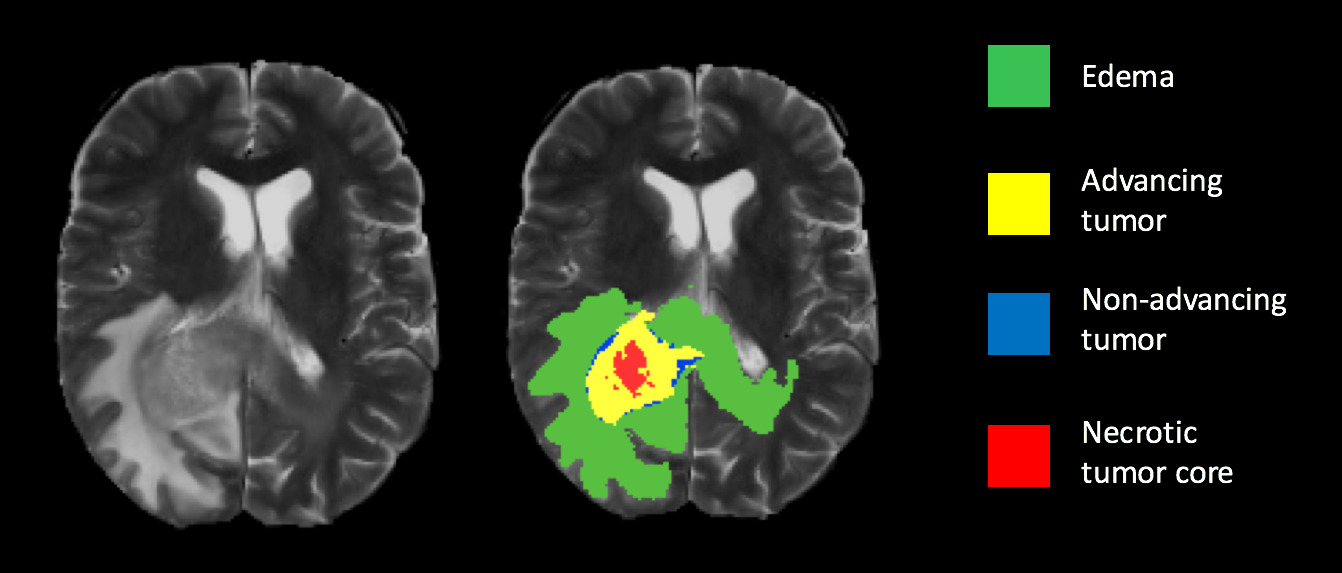
\includegraphics[
                    height=4.2cm,
                    trim={0 0 13.8cm 0},
                    clip
                ]{data/tumor.png}
            };
        \end{tikzpicture}
    }
    \only<15>{
        \centering
        \begin{tikzpicture}
            \node[] at (-5.25, 3.5) {};
            \node[] at (5.25, -3.5) {};
            \node[anchor=west] at (-5.25, 0) {
                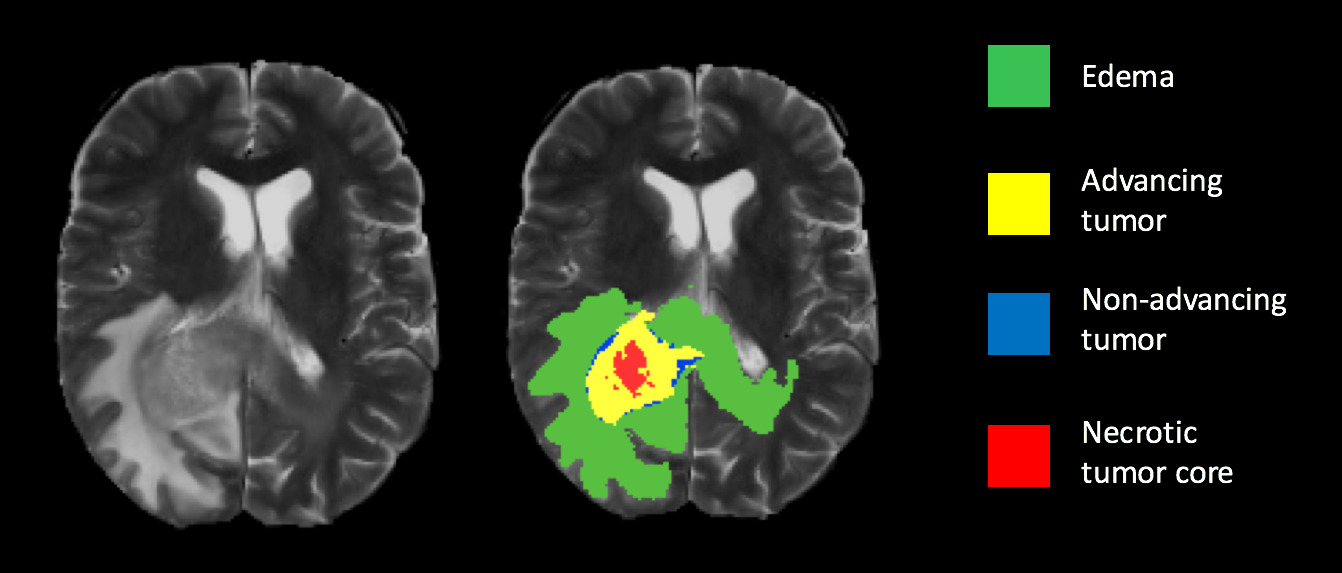
\includegraphics[height=4.2cm]{data/tumor.png}
            };
        \end{tikzpicture}
    }
    \only<16-17>{
        \begin{tikzpicture}
            \node[] at (-5.5, 3.5) {};
            \node[] at (5, -3.5) {};
            \node[] at (0, 0) {
                
\includegraphics[width=5cm]{data/dog.png}
            };
            \draw[orange, thick] (-0.8, 1.4) -- (1.7, 1.4) -- (1.7, -1.8) -- (-0.8, -1.8) -- cycle;

            \only<17>{
                \node[anchor=south, orange] at (0.45, 1.4) {Dog};
                \node[anchor=south, orange] at (-0.8, 1.4) {\footnotesize{(-0.8, 1.4)}};
                \node[anchor=south, orange] at (1.7, 1.4) {\footnotesize{(1.7, 1.4)}};
                \node[anchor=north, orange] at (-0.8, -1.8) {\footnotesize{(-0.8, -1.8)}};
                \node[anchor=north, orange] at (1.7, -1.8) {\footnotesize{(1.7, -1.8)}};
            }

        \end{tikzpicture}
    }
    \only<18-19>{
        \begin{tikzpicture}
            \node[] at (-5.5, 3.5) {};
            \node[] at (5, -3.5) {};

            \node[inner sep=0pt, draw=black] at (0, 1.5) {
                
\includegraphics[width=3.5cm]{data/robot.png}
            };
            \only<19>{
                \node[inner sep=0pt, draw=black] at (0, -2) {
                    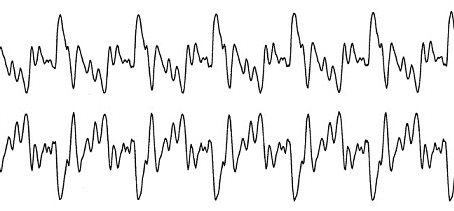
\includegraphics[width=5cm]{data/sound.png}
                };
            }
        \end{tikzpicture}
    }
    \only<20>{
        \textbf{Different types of outputs $\mathbf{y}$ require us to use different mathematical formulations of the problem we want to solve.}
        \begin{itemize}
            \item Problems with quantitative outputs are solved via regression, often by minimizing the mean squared error
            \item Problems with qualitative outputs are solved by classification, often to maximize accuracy
            \item Ordinal regression falls between the two, with qualitative classes that have some kind of order
            \item A variety of other types of problems can be seen as special cases of these two
        \end{itemize}
    }
\end{frame}

\newsavebox{\linreg}
\sbox{\linreg}{
    \begin{tikzpicture}
        \begin{axis}[
            xmin=30,
            xmax=240,
            ymin=3,
            ymax=50,
            width=5.2cm,
            height=5.2cm,
            ylabel=mpg,
            xlabel=horsepower
        ]
            \addplot[
                only marks,
                opacity=0.3
            ] table [
                col sep=comma,
                x=horsepower,
                y=mpg
            ] {data/Auto.csv};
            \addplot[
                domain=30:240,
                samples=100,
                color=red,
                thick
            ] {39.93 - 0.1578*x};
        \end{axis}
    \end{tikzpicture}
}

\newsavebox{\residuals}
\sbox{\residuals}{
    \begin{tikzpicture}
        \begin{axis}[
            xmin=30,
            xmax=240,
            ymin=-20,
            ymax=20,
            width=5.2cm,
            height=5.2cm,
            ylabel=$y-\hat{y}$,
            xlabel=horsepower
        ]
            \addplot[
                only marks,
                opacity=0.3
            ] table [
                col sep=comma,
                x=horsepower,
                y=residuals
            ] {data/residuals.csv};
            \addplot[
                domain=30:240,
                samples=100,
                color=red,
                thick
            ] {0};
        \end{axis}
    \end{tikzpicture}
}
\section{Linear regression (via ordinary least squares)}

\begin{frame}{Linear regression (via ordinary least squares)}
    \only<1-15>{
        \begin{tikzpicture}
            \begin{axis}[
                xtick pos=bottom,
                ytick pos=left,
                xmin=-70,
                xmax=140,
                ymin=3,
                ymax=50,
                xlabel=x (horsepower),
                ylabel=y (mpg),
                height=6.8cm,
                width=10.7cm
            ]
                \only<1-3,6>{
                    \addplot[
                        only marks,
                        opacity=0.5,
                        cyan
                    ] table [
                        col sep=comma,
                        x expr=\thisrow{horsepower}-100,
                        y=mpg
                    ] {data/Auto.csv};
                }
                \only<2>{
                    \node[text=red] at (rel axis cs: 0.7, 0.8) {
                        $\hat{y}=\beta_0+\beta_1x$
                    };
                }
                \only<3-7>{
                    \node[text=red, anchor=west] at (rel axis cs: 0.533, 0.8) {
                        $\hat{y}=24.23-0.157x$
                    };
                }
                \only<3-15>{
                    \addplot[
                        domain=-70:140,
                        samples=2,
                        color=red,
                        thick
                    ] {39.93 - 0.1578*(x+100)};
                }
                \only<4-5,7-15>{
                    \addplot[
                        only marks,
                        opacity=0.1,
                        cyan
                    ] table [
                        col sep=comma,
                        x expr=\thisrow{horsepower}-100,
                        y=mpg
                    ] {data/Auto.csv};
                }
                \only<4>{
                    \draw[] (axis cs: 0, 3) -- (axis cs: 0, 50);
                    \draw[densely dotted, thick] (axis cs: -70, 24.23) -- (axis cs: 140, 24.23);
                }
                \only<5>{
                    \draw[thick] (axis cs: 0, 24.23) -- (axis cs: 20, 24.23) -- (axis cs: 20, 21.09);
                }
                \only<6>{
                    \addplot[
                        domain=-70:140,
                        samples=2,
                        color=blue,
                        thick
                    ] {26 - 0.1*x};

                    \node[text=blue, anchor=west] at (rel axis cs: 0.533, 0.73) {
                        $\hat{y}=26-0.1x$
                    };
                }

                \only<8-9>{
                    \draw[dashed] (axis cs: 15, 3) -- (axis cs: 15, 50);
                    \node[anchor=south, draw=black, fill=white, inner sep=2pt] at (axis cs: 15, 5) {\small{15}};
                }
                \only<8-9>{
                    \node[text=red, anchor=west] at (rel axis cs: 0.533, 0.8) {
                        $\hat{y}=24.23-0.157*15$
                    };
                }
                \only<9-15>{
                    \node[circle, draw=red, inner sep=1.5pt, fill=red, opacity=0.5] (yhat) at (axis cs: 15, 21.78) {};
                }
                \only<9>{
                    \node[text=red, anchor=west, font=\footnotesize] at ($ (yhat.east) + (2, 0) $) {21.78};
                }
                \only<10-13>{
                    \node[text=red, anchor=north, font=\footnotesize] at (yhat.south) {$\hat{y}$};
                }
                \only<11-15>{
                    \node[circle, draw=cyan, inner sep=1.5pt, fill=cyan, opacity=0.5] (y) at (axis cs: 15, 28.9) {};
                }
                \only<11-13>{
                    \node[text=cyan, anchor=south, font=\footnotesize] at (y.north) {$y$};
                }
                \only<12>{
                    \draw[stealth-stealth] (yhat) -- (y) node [midway, right, font=\footnotesize] {residual};
                }
                \only<12-15>{
                    \node[text depth=0] at (rel axis cs: 0.8, 0.8) {$y-\hat{y}$};
                }
                \only<13-15>{
                    \draw[] (axis cs: 15, 21.78) -- (axis cs: 15, 28.9) -- (axis cs: 15 + 2.8*7.12, 28.9) -- (axis cs: 15 + 2.8*7.12, 21.78) -- cycle;
                    \node[text depth=0] at (rel axis cs: 0.86, 0.8) {$)^2$};
                    \node[text depth=0] at (rel axis cs: 0.745, 0.7975) {$($};
                }
                \only<14-15>{
                    \node[text=red, anchor=north, font=\footnotesize] at (yhat.south) {$\hat{y}_1$};
                    \node[text=cyan, anchor=south, font=\footnotesize] at (y.north) {$y_1$};

                    \node[circle, draw=red, inner sep=1.5pt, fill=red, opacity=0.5] (yhat) at (axis cs: 98, 8.844) {};
                    \node[text=red, anchor=north, font=\footnotesize] at (yhat.south) {$\hat{y}_3$};
                    \node[circle, draw=cyan, inner sep=1.5pt, fill=cyan, opacity=0.5] (y) at (axis cs: 98, 15) {};
                    \node[text=cyan, anchor=south, font=\footnotesize] at (y.north) {$y_3$};
                    \draw[] (axis cs: 98, 8.844) -- (axis cs: 98, 15) -- (axis cs: 98 + 2.8*6.15, 15) -- (axis cs: 98 + 2.8*6.15, 8.844) -- cycle;

                    \node[circle, draw=red, inner sep=1.5pt, fill=red, opacity=0.5] (yhat) at (axis cs: 40, 17.95) {};
                    \node[text=red, anchor=south, font=\footnotesize] at (yhat.north) {$\hat{y}_2$};
                    \node[circle, draw=cyan, inner sep=1.5pt, fill=cyan, opacity=0.5] (y) at (axis cs: 40, 14) {};
                    \node[text=cyan, anchor=north, font=\footnotesize] at (y.south) {$y_2$};
                    \draw[] (axis cs: 40, 17.95) -- (axis cs: 40, 14) -- (axis cs: 40 + 2.8*3.95, 14) -- (axis cs: 40 + 2.8*3.95, 17.95) -- cycle;

                    \node[circle, draw=red, inner sep=1.5pt, fill=red, opacity=0.5] (yhat) at (axis cs: -39.7, 30.4629) {};
                    \node[text=red, anchor=south, font=\footnotesize] at (yhat.north) {$\hat{y}_0$};
                    \node[circle, draw=cyan, inner sep=1.5pt, fill=cyan, opacity=0.5] (y) at (axis cs: -39.7, 27) {};
                    \node[text=cyan, anchor=north, font=\footnotesize] at (y.south) {$y_0$};
                    \draw[] (axis cs: -39.7, 30.4629) -- (axis cs: -39.7, 27) -- (axis cs: -39.7 + 2.8*3.4629, 27) -- (axis cs: -39.7 + 2.8*3.4629, 30.4629) -- cycle;

                    \node[text depth=0, font=\tiny] at (rel axis cs: 0.841, 0.78) {$i$};
                    \node[text depth=0, font=\tiny] at (rel axis cs: 0.775, 0.78) {$i$};
                }
                \only<14>{
                    \node[text depth=0, anchor=east] at (rel axis cs: 0.75, 0.82) {$MSE=\dfrac{1}{n}\sum\limits_{i=0}^n$};
                }
                \only<15>{
                    \node[text depth=0, anchor=east] at (rel axis cs: 0.75, 0.82) {$RSS=\sum\limits_{i=0}^n$};
                }
            \end{axis}
        \end{tikzpicture}\\
    }
    \only<16>{
        \textbf{Linear regression}: Models the relationship between input $x$ and output $y$ by finding the linear model $\hat{y}=\beta_0+\beta_1x$ that minimizes the residual sum of squares (RSS).
        \begin{itemize}
            \item $\beta_0$ refers to the intercept (or offset) of the model
            \item $\beta_1$ refers to the slope of the model
        \end{itemize}
    }
    \centering
\end{frame}

\newcommand{\modelchange}[1]{
    \begin{tikzpicture}
        \begin{axis}[
            height=5.5cm,
            width=5.5cm,
            xlabel=x (horsepower),
            ylabel=y (mpg),
            ymin=3,
            ymax=50,
            xmin=30,
            xmax=240,
            xtick pos=bottom,
            ytick pos=left
        ]

        \addplot[
            domain=30:240,
            samples=2,
            cyan,
            thick
        ] {39.93 - 0.21*x};
        \addplot[
            domain=30:240,
            samples=2,
            red,
            thick
        ] {39.93 - 0.15*x};
        \addplot[
            domain=30:240,
            samples=2,
            blue,
            thick
        ] {39.93 - 0.07*x};

        \ifnum#1=0
            \node[anchor=west, font=\scriptsize, text=blue] at (rel axis cs: 0.17, 0.94) {
                $\hat{f}(x)=39.93-0.07x$
            };
            \node[anchor=west, font=\scriptsize, text=red] at (rel axis cs: 0.17, 0.84) {
                $\hat{f}(x)=39.93-0.15x$
            };
            \node[anchor=west, font=\scriptsize, text=cyan] at (rel axis cs: 0.17, 0.74) {
                $\hat{f}(x)=39.93-0.21x$
            };
        \fi

        \ifnum#1<4
            \ifnum#1>0
                \node[anchor=west, font=\scriptsize, text=blue] at (rel axis cs: 0.17, 0.94) {
                    $\hat{f}(150)=39.93-0.07*150$
                };
                \node[anchor=west, font=\scriptsize, text=red] at (rel axis cs: 0.17, 0.84) {
                    $\hat{f}(150)=39.93-0.15*150$
                };
                \node[anchor=west, font=\scriptsize, text=cyan] at (rel axis cs: 0.17, 0.74) {
                    $\hat{f}(150)=39.93-0.21*150$
                };
                \node[circle, draw=blue, inner sep=2pt, opacity=0.5, fill=blue] (bluey) at (axis cs: 150, 29.43) {};
                \node[circle, draw=red, inner sep=2pt, opacity=0.5, fill=red] (redy) at (axis cs: 150, 17.43) {};
                \node[circle, draw=teal, inner sep=2pt, opacity=0.5, fill=teal] (tealy) at (axis cs: 150, 8.43) {};

                \ifnum#1<3
                    \node[anchor=south, text=blue] at (bluey.north) {\scriptsize{$\hat{y}$}};
                    \node[anchor=north, text=red] at (redy.south) {\scriptsize{$\hat{y}$}};
                    \node[anchor=north, text=teal] at (tealy.south) {\scriptsize{$\hat{y}$}};
                \fi
            \fi

            \ifnum#1=2
                \node[circle, draw=black, inner sep=2pt, opacity=0.5, fill=black, label=right:\scriptsize{$y$}] at (axis cs: 150, 22.43) {};
            \fi
            \ifnum#1>2
                \node[circle, draw=black, inner sep=2pt, opacity=0.5, fill=black] at (axis cs: 150, 22.43) {};
                \draw[blue, densely dotted, thick] (axis cs: 150, 29.43) -- (axis cs: 150, 22.43) -- (axis cs: 150 + 4.5*7, 22.43) -- (axis cs: 150 + 4.5*7, 29.43) -- cycle;
                \draw[red, densely dotted, thick] (axis cs: 150, 17.43) -- (axis cs: 150, 22.43) -- (axis cs: 150 + 4.5*5, 22.43) -- (axis cs: 150 + 4.5*5, 17.43) -- cycle;
                \draw[teal, densely dotted, thick] (axis cs: 150, 8.43) -- (axis cs: 150, 22.43) -- (axis cs: 150 + 4.5*14, 22.43) -- (axis cs: 150 + 4.5*14, 8.43) -- cycle;
            \fi
        \fi
        \ifnum#1>3
            \addplot[
                only marks,
                black,
                opacity=0.15
            ] table [
                col sep=comma,
                x=horsepower,
                y=mpg
            ] {data/Auto.csv};

            \node[anchor=west, font=\scriptsize, text=blue] at (rel axis cs: 0.3, 0.93) {
                $\hat{f}(x)=39.93-0.07x$
            };
            \node[anchor=west, font=\scriptsize, text=red] at (rel axis cs: 0.3, 0.83) {
                $\hat{f}(x)=39.93-0.15x$
            };
            \node[anchor=west, font=\scriptsize, text=cyan] at (rel axis cs: 0.3, 0.73) {
                $\hat{f}(x)=39.93-0.21x$
            };
        \fi
        \end{axis}
    \end{tikzpicture}
}

\newcommand{\losschange}[1]{
    \begin{tikzpicture}
        \begin{axis}[
            height=5.5cm,
            width=5.5cm,
            xlabel=$\beta_1$,
            ylabel=Squared error,
            xtick pos=bottom,
            ytick pos=left,
            xmin=0.02,
            xmax=0.23,
            ymin=0,
            ymax=300,
            xtick={0.05, 0.1, 0.15, 0.2},
            xticklabels={0.05, 0.1, 0.15, 0.2}
        ]

            \ifnum#1<2
                \node[circle, draw=blue, inner sep=2pt, opacity=0.5, fill=blue] at (axis cs: 0.07, 49) {};
                \node[circle, draw=red, inner sep=2pt, opacity=0.5, fill=red] at (axis cs: 0.15, 25) {};
                \node[circle, draw=teal, inner sep=2pt, opacity=0.5, fill=teal] at (axis cs: 0.21, 196) {};

                \ifnum#1>0
                    \addplot[
                        domain=0:0.25,
                        samples=100,
                        color=black,
                        thick
                    ] {((39.93-150*x)-22.43)^2};
                \fi
            \fi

            \ifnum#1>1
                \node[circle, draw=blue, inner sep=2pt, opacity=0.5, fill=blue] at (axis cs: 0.07, 59) {};
                \node[circle, draw=red, inner sep=2pt, opacity=0.5, fill=red] at (axis cs: 0.15, 35) {};
                \node[circle, draw=teal, inner sep=2pt, opacity=0.5, fill=teal] at (axis cs: 0.21, 206) {};

                \addplot[
                    domain=0:0.25,
                    samples=100,
                    color=black,
                    thick
                ] {10+((39.93-150*x)-22.43)^2};
            \fi
        \end{axis}
    \end{tikzpicture}
}

\begin{frame}{Fitting a linear regression model}
    \begin{tikzpicture}
        \node[] at (-5.25, -3) {};
        \node[] at (5.25, 3) {};

        \only<1-4>{
            \node[font=\LARGE] at (0, 0.1) {
                $\alert<4>{\hat{y}}=\alert<2>{\beta_0}+\alert<2>{\beta_1}x$
            };
        }
        \only<3-4>{
            \node[font=\LARGE] at (0, -1.1) {
                $RSS=\sum\limits_{i=0}^{n}(y_i-\alert<4>{\hat{y}}_i)^2$
            };
        }
        \only<5>{
            \node[font=\LARGE] at (0, -0.5) {
                $RSS=\sum\limits_{i=0}^{n}(y_i-\beta_0+\beta_1x_i)^2$
            };
        }
        \only<6>{
            \node[] at (-2.675, 0) {
                \modelchange{0}
            };
        }
        \only<7>{
            \node[] at (-2.675, 0) {
                \modelchange{1}
            };
        }
        \only<8>{
            \node[] at (-2.675, 0) {
                \modelchange{2}
            };
        }
        \only<9-11>{
            \node[] at (-2.675, 0) {
                \modelchange{3}
            };
        }
        \only<10>{
            \node[] at (2.675, 0.145) {
                \losschange{0}
            };
        }
        \only<11>{
            \node[] at (2.675, 0.145) {
                \losschange{1}
            };
        }
        \only<12-13>{
            \node[] at (-2.675, 0) {
                \modelchange{4}
            };
        }
        \only<13>{
            \node[] at (2.675, 0.145) {
                \losschange{2}
            };
        }
    \end{tikzpicture}
\end{frame}

\newsavebox{\multilinreg}
\sbox{\multilinreg}{
    \begin{tikzpicture}
        \begin{axis}[
            width=8cm,
            height=7cm, % Size of the plot
            xlabel={Horsepower ($x_1$)},
            ylabel={Weight ($x_2$)},
            zlabel={Miles per gallon (y)},
            view={25}{25}, % Adjust viewing angle colormap/cool,
            xmin=30,
            xmax=240,
            ymin=1500,
            ymax=5000,
            zmin=3,
            zmax=50,
            xlabel style={sloped},
            ylabel style={sloped},
            xmajorgrids=true,
            ymajorgrids=true,
            zmajorgrids=true,
            xtick style={draw=none},
            ytick style={draw=none},
            ztick style={draw=none}
        ]
            \addplot3[
                surf,
                samples=20,
                domain=30:240,
                y domain=1500:5000,
            ] {45.64-0.04*x-0.005*y};
            \addplot3[
                only marks,
                mark size=2.5pt,
                opacity=0.25
            ] table [
                x=horsepower,
                y=weight,
                z=mpg,
                col sep=comma
            ] {data/Auto.csv};
        \end{axis}
    \end{tikzpicture}
}

\begin{frame}{Multivariate linear regression}
    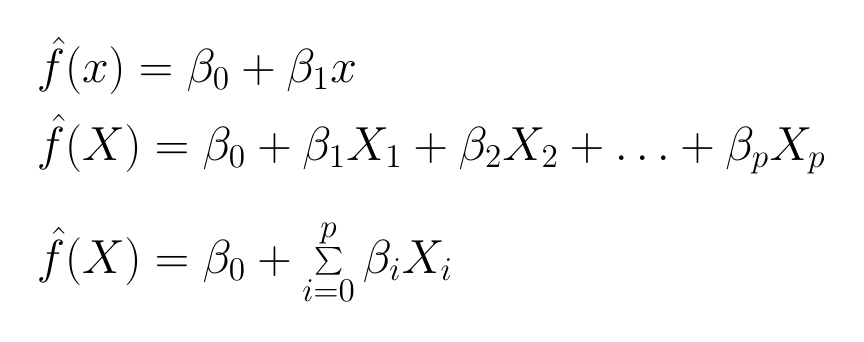
\begin{tikzpicture}
        \visible<1-3>{
            \node[font=\LARGE, anchor=west] at (-4, 1) {
                $\hat{f}(x)=\beta_0+\beta_1x$
            };
        }
        \visible<2-3>{
            \node[font=\LARGE, anchor=west] at (-4, 0) {
                $\hat{f}(X)=\beta_0+\beta_1X_1+\beta_2X_2+\ldots+\beta_pX_p$
            };
        }
        \visible<3>{
            \node[font=\LARGE, anchor=west] at (-4, -1.5) {
                $\hat{f}(X)=\beta_0+\sum\limits_{i=0}^p\beta_iX_i$
            };
        }
        \visible<4>{
            \node[] at (0, 0) {
                \usebox{\multilinreg}
            };
        }
    \end{tikzpicture}
\end{frame}

\newcommand{\binaryplot}[1]{
    \begin{tikzpicture}
        \begin{axis}[
            xmin=-0.5,
            xmax=1.5,
            xtick={0, 1},
            xticklabels={Ford, Chevrolet},
            ylabel=mpg,
            height=7cm,
            width=7cm
        ]
            \addplot[
                only marks,
                fill=blue,
                opacity=0.6
            ] coordinates {
                (-0.065, 18)
                (-0.080, 15)
                (-0.038, 18)
                (-0.139, 16)
                (0.028, 17)
                (-0.140, 15)
                (-0.149, 14)
                (0.137, 14)
                (0.043, 14)
                (-0.101, 15)
                (0.007, 15)
                (-0.145, 14)
                (-0.106, 15)
                (-0.013, 14)
                (-0.120, 24)
                (0.150, 22)
                (-0.166, 18)
                (-0.052, 21)
                (0.031, 27)
            };
            \addplot[
                only marks,
                fill=red,
                opacity=0.6
            ] coordinates {
                (0.985, 38)
                (0.943, 36)
                (1.085, 36)
                (0.971, 36)
                (0.990, 34)
                (1.029, 38)
                (0.958, 32)
                (1.018, 38)
                (1.054, 25)
                (1.064, 38)
                (1.070, 26)
                (0.938, 22)
                (1.131, 32)
                (1.009, 36)
                (0.835, 27)
                (1.109, 27)
                (1.032, 44)
                (1.142, 32)
                (1.115, 28)
                (1.009, 31)
            };
            \ifnum#1=2
                \draw[thick, dashed] (axis cs: -0.3, 17.158) -- (axis cs: 0.3, 17.158);
                \node[anchor=south east, inner sep=1pt] at (axis cs: 0.3, 17.158) {\small{17.1}};
                \draw[thick, dashed] (axis cs: 0.7, 32.8) -- (axis cs: 1.3, 32.8);
                \node[anchor=south west, inner sep=1pt] at (axis cs: 0.7, 32.8) {\small{32.8}};
            \fi
        \end{axis}
    \end{tikzpicture}
}

\newsavebox{\multilevel}
\savebox{\multilevel}{
    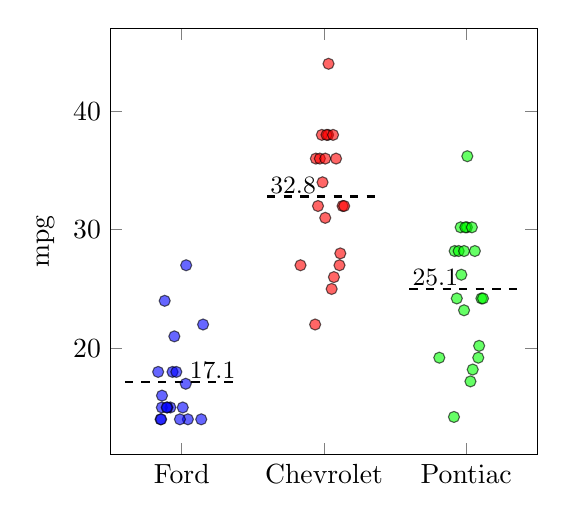
\begin{tikzpicture}
        \begin{axis}[
            xmin=-0.5,
            xmax=2.5,
            xtick={0, 1, 2},
            xticklabels={Ford, Chevrolet, Pontiac},
            ylabel=mpg,
            height=7cm,
            width=7cm
        ]
            \addplot[
                only marks,
                fill=blue,
                opacity=0.6
            ] coordinates {
                (-0.065, 18)
                (-0.080, 15)
                (-0.038, 18)
                (-0.139, 16)
                (0.028, 17)
                (-0.140, 15)
                (-0.149, 14)
                (0.137, 14)
                (0.043, 14)
                (-0.101, 15)
                (0.007, 15)
                (-0.145, 14)
                (-0.106, 15)
                (-0.013, 14)
                (-0.120, 24)
                (0.150, 22)
                (-0.166, 18)
                (-0.052, 21)
                (0.031, 27)
            };
            \addplot[
                only marks,
                fill=red,
                opacity=0.6
            ] coordinates {
                (0.985, 38)
                (0.943, 36)
                (1.085, 36)
                (0.971, 36)
                (0.990, 34)
                (1.029, 38)
                (0.958, 32)
                (1.018, 38)
                (1.054, 25)
                (1.064, 38)
                (1.070, 26)
                (0.938, 22)
                (1.131, 32)
                (1.009, 36)
                (0.835, 27)
                (1.109, 27)
                (1.032, 44)
                (1.142, 32)
                (1.115, 28)
                (1.009, 31)
            };
            \addplot[
                only marks,
                fill=green,
                opacity=0.6
            ] coordinates {
                (1.961, 30.200)
                (1.919, 28.200)
                (2.061, 28.200)
                (1.947, 28.200)
                (1.966, 26.200)
                (2.005, 30.200)
                (1.934, 24.200)
                (1.994, 30.200)
                (2.030, 17.200)
                (2.040, 30.200)
                (2.046, 18.200)
                (1.914, 14.200)
                (2.107, 24.200)
                (1.985, 28.200)
                (1.811, 19.200)
                (2.085, 19.200)
                (2.008, 36.200)
                (2.118, 24.200)
                (2.091, 20.200)
                (1.985, 23.200)
            };

            \draw[thick, dashed] (axis cs: -0.4, 17.158) -- (axis cs: 0.4, 17.158);
            \node[anchor=south east, inner sep=1pt] at (axis cs: 0.4, 17.158) {\small{17.1}};
            \draw[thick, dashed] (axis cs: 0.6, 32.8) -- (axis cs: 1.4, 32.8);
            \node[anchor=south west, inner sep=1pt] at (axis cs: 0.6, 32.8) {\small{32.8}};
            \draw[thick, dashed] (axis cs: 1.6, 25) -- (axis cs: 2.4, 25);
            \node[anchor=south west, inner sep=1pt] at (axis cs: 1.6, 25) {\small{25.1}};

        \end{axis}
    \end{tikzpicture}
}

\newcommand{\combinationplot}[1]{
    \begin{tikzpicture}
        \begin{axis}[
            xtick pos=bottom,
            ytick pos=left,
            xmin=30,
            xmax=240,
            ymin=3,
            ymax=50,
            xlabel=x (horsepower),
            ylabel=y (mpg),
            height=6.5cm,
            width=10cm
        ]
            \addplot[
                only marks,
                opacity=0.5,
                cyan
            ] table [
                col sep=comma,
                x=horsepower,
                y=mpg
            ] {data/Auto.csv};

            \ifnum#1=1
                \addplot[
                    domain=30:240,
                    samples=100,
                    color=red,
                    thick
                ] {40 - 0.1566*x};
                \addplot[
                    domain=30:240,
                    samples=100,
                    color=blue,
                    thick
                ] {40 - 0.1566*x-1.85};
            \fi
            \ifnum#1=2
                \addplot[
                    domain=30:240,
                    samples=100,
                    color=red,
                    thick
                ] {40 - 0.1566*x};
                \addplot[
                    domain=30:240,
                    samples=100,
                    color=blue,
                    thick
                ] {38 - 0.13*x-1.85};
            \fi
        \end{axis}
    \end{tikzpicture}
}

\begin{frame}{Categorical variables}
    \begin{tikzpicture}
        \node[] at (-5.25, -3.5) {};
        \node[] at (5.25, 3.5) {};

        \only<1>{
            \node[] at (0, 0) {
                \begin{tabular}{cc}
                    \textbf{mpg}&\textbf{manufacturer}\\
                    36&Chevrolet\\
                    15&Ford\\
                    25&Chevrolet\\
                    26&Chevrolet\\
                    17&Ford\\
                    15&Ford\\
                    32&Chevrolet\\
                    14&Ford\\
                    14&Ford\\
                    28&Chevrolet\\
                \end{tabular}
            };
            \node[] at (0, -3.1) {
                $\widehat{\text{mpg}}=\beta_0+\beta_1\times\text{manufacturer}$
            };
        }
        \only<2>{
            \node[] at (0, 0) {
                \begin{tabular}{ccc}
                    \textbf{mpg}&\textbf{manufacturer}&\textbf{chevrolet}\\
                    36&Chevrolet&1\\
                    15&Ford&0\\
                    25&Chevrolet&1\\
                    26&Chevrolet&1\\
                    17&Ford&0\\
                    15&Ford&0\\
                    32&Chevrolet&1\\
                    14&Ford&0\\
                    14&Ford&0\\
                    28&Chevrolet&1\\
                \end{tabular}
            };
            \node[] at (0, -3.1) {
                $\widehat{\text{mpg}}=\beta_0+\beta_1\times\text{chevrolet}$
            };
        }
        \only<3>{
            \node[] at (0, 0) {
                \binaryplot{1}
            };
        }
        \only<4-5>{
            \node[] at (0, 0) {
                \binaryplot{2}
            };
        }
        \only<5>{
            \node[rotate=45, draw=black, fill=white] at (0.5, 0) {
                \textbf{\Huge{Blackboard!}}
            };
        }
        \only<6>{
            \node[] at (0, 0) {
                \begin{tabular}{cc}
                    \textbf{mpg}&\textbf{manufacturer}\\
                    36&Chevrolet\\
                    15&Ford\\
                    25&Chevrolet\\
                    26&Pontiac\\
                    17&Ford\\
                    15&Ford\\
                    32&Pontiac\\
                    14&Ford\\
                    14&Pontiac\\
                    28&Chevrolet\\
                \end{tabular}
            };
            \node[] at (0, -3.5) {
                $\widehat{\text{mpg}}=\beta_0+\beta_1\times\text{manufacturer}$
            };
        }
        \only<7>{
            \node[] at (0, 0) {
                \begin{tabular}{cccc}
                    \textbf{mpg}&\textbf{manufacturer}&\textbf{chevrolet}&\textbf{pontiac}\\
                    36&Chevrolet&1&0\\
                    15&Ford&0&0\\
                    25&Chevrolet&1&0\\
                    26&Pontiac&0&1\\
                    17&Ford&0&0\\
                    15&Ford&0&0\\
                    32&Pontiac&0&1\\
                    14&Ford&0&0\\
                    14&Pontiac&0&1\\
                    28&Chevrolet&1&0\\
                \end{tabular}
            };
            \node[] at (0, -3.25) {
                $\widehat{\text{mpg}}=\beta_0+\beta_1\times\text{chevrolet}+\beta_2\times\text{pontiac}$
            };
        }
        \only<8>{
            \PythonInputNode{1}{(-4, 2)}{pythonnode}{0.9\textwidth}{7}{
                import pandas as pd^^J
                ^^J
                df = pd.DataFrame(...)^^J
                print(f'Columns before: \{df.columns.values\}')^^J
                df = pd.get_dummies(df)^^J
                print(f'Columns after: \{df.columns.values\})^^J
            }
            \PythonOutputNode{1}{(-3.895, 0)}{out}{0.79\textwidth}{7}{
                Columns before: ['manufacturer']^^J
                Columns after: ['manufacturer_chevrolet' 'manufacturer_ford']^^J
            }
        }
        \only<9>{
            \node[] at (0, 0) {
                \usebox{\multilevel}
            };
        }
        \only<10-11>{
            \node[] at (0, 0.4) {
                \begin{tabular}{ccc}
                    \textbf{mpg}&\textbf{chevrolet}&\textbf{horsepower}\\
                    36&1&130\\
                    15&0&165\\
                    25&1&150\\
                    26&1&150\\
                    17&0&140\\
                    15&0&198\\
                    32&1&220\\
                    14&0&215\\
                    14&0&225\\
                    28&1&212\\
                \end{tabular}
            };
        }
        \only<10>{
            \node[] at (0, -3) {
                $\widehat{\text{mpg}}=\beta_0+\beta_1\times\text{chevrolet}+\beta_2\times\text{horsepower}$
            };
        }
        \only<11>{
            \node[align=center] at (0, -3) {
                $\widehat{mpg}=
                \begin{cases}
                    \beta_0+\beta_1+\beta_2\times\text{horsepower} & \text{if chevrolet}\\
                    \beta_0+\beta_2\times\text{horsepower} & \text{else}\\
                \end{cases}$
            };

        }
        \only<12>{
            \node[] at (0, 0.5) {
                \combinationplot{1}
            };
            \node[align=center] at (0, -3.3) {
                $\widehat{mpg}=
                \begin{cases}
                    \textcolor{blue}{\beta_0+\beta_1+\beta_2\times\text{horsepower}} & \text{if chevrolet}\\
                    \textcolor{red}{\beta_0+\beta_2\times\text{horsepower}} & \text{else}\\
                \end{cases}$
            };
        }
        \only<13-14>{
            \node[] at (0, 0.5) {
                \combinationplot{2}
            };
        }
        \only<14>{
            \node[align=center] at (0, -3.1) {
                $\widehat{mpg}=\beta_0+\beta_1\times\text{chevrolet}+\beta_2\times\text{horsepower}$\\
                $+\beta_3\times\text{chevrolet}\times\text{horsepower}$
            };
        }
    \end{tikzpicture}
\end{frame}

\newcommand{\cisplot}[1]{
    \begin{tikzpicture}
        \begin{axis}[
            xtick pos=bottom,
            ytick pos=left,
            xmin=30,
            xmax=240,
            ymin=3,
            ymax=50,
            xlabel=Horsepower,
            ylabel=Miles per gallon,
            height=6.5cm,
            width=10.5cm
        ]
            \addplot[
                domain=30:240,
                samples=100,
                color=red,
                thick
            ] {40 - 0.1566*x};

            \ifnum#1>1
                \addplot[
                    only marks,
                ] coordinates {
                    (105, 23.5)
                };
                \draw[|-|, dashed] (axis cs: 105, 17.5) -- (axis cs: 105, 29.5);
                \node[anchor=south, align=center, font=\scriptsize\linespread{0.8}\selectfont] at (axis cs: 105, 29.5) {
                    Prediction\\
                    interval
                };
            \fi

            \ifnum#1>2
                \addplot[
                    only marks,
                    opacity=0.2
                ] coordinates {
                    (140, 22)
                    (140, 21)
                    (140, 19)
                    (140, 18)
                    (140, 15)
                };

                \draw[|-|, densely dotted, red, thick] (axis cs: 140, 16) -- (axis cs: 140, 20);
                \node[anchor=south, align=center, red, font=\scriptsize\linespread{0.8}\selectfont] at (axis cs: 140, 23) {
                    Confidence\\
                    interval
                };
            \fi

        \end{axis}
    \end{tikzpicture}
}

\begin{frame}{Confidence intervals}
    \begin{tikzpicture}
        \node[] at (-5.25, -3.5) {};
        \node[] at (5.25, 3.5) {};

        \only<1>{
            \node[] at (0, 0) {
                \cisplot{1}
            };
        }
        \only<2>{
            \node[] at (0, 0) {
                \cisplot{2}
            };
        }
        \only<3>{
            \node[] at (0, 0) {
                \cisplot{3}
            };
        }
        \only<4>{
            \RInputNode{(-4.5, 2)}{in1}{0.8\textwidth}{7}{
predict(fit, newdata=data.frame(horsepower=105),^^J
{ }{ }{ }{ }{ }{ }{ }{ }interval='prediction', level=0.95)^^J
            }
            \RInputNode{(-4.5, 1)}{out1}{0.8\textwidth}{7}{
{ }{ }{ }{ }{ }fit{ }{ }{ }{ }lwr{ }{ }{ }{ }upr^^J
1 23.535 17.158 29.912^^J
            }
            \RInputNode{(-4.5, -1)}{in2}{0.8\textwidth}{7}{
predict(fit, newdata=data.frame(horsepower=105),^^J
{ }{ }{ }{ }{ }{ }{ }{ }interval='confidence', level=0.95)^^J
            }
            \RInputNode{(-4.5, -2)}{out1}{0.8\textwidth}{7}{
                { }{ }{ }{ }{ }fit{ }{ }{ }{ }lwr{ }{ }{ }{ }upr^^J
                1 23.535 23.023 24.047^^J
            }
        }
        \only<5>{
            \PythonInputNode{1}{(-4.5, 2)}{pythonnode}{0.95\textwidth}{7}{
                import statsmodels.api as sm^^J
                ^^J
                model = sm.OLS(df['mpg'], sm.add_constant(df[['horsepower']]))^^J
                fit = model.fit()^^J
                new_input = sm.add_constant(pd.DataFrame(\{'horsepower': [105, 106]\}))^^J
                intervals = fit.get_prediction(new_input).summary_frame()^^J
                print(intervals)^^J
            }
            \PythonOutputNode{1}{(-4.395, -0.5)}{out}{0.882\textwidth}{7}{
                mean   mean_se  mean_ci_lower  mean_ci_upper  obs_ci_lower  obs_ci_upper^^J
                0  24.467077  0.251262      23.973079      24.961075     14.809396     34.124758^^J
                1  31.096556  0.398740      30.312607      31.880505     21.419710     40.773402^^J
            }
        }
        \only<6>{
            \node[align=center] at (0, 0) {
                Why do we need both of these?\\
                Where are they useful (e.g. what is most useful in\\
                a scientific publication versus a business setting)?\\
            };
        }

        \only<7>{
            \node[] at (0, 1) {
                \Huge{\emoji{partying-face}}
            };

            \node[] at (0, -1) {
                \scriptsize{\url{http://localhost:8888/notebooks/notebooks\%2FLinear\%20regression.ipynb}}
            };
        }
    \end{tikzpicture}
\end{frame}

\begin{frame}{Linear regression: Summary}
    \textbf{Linear regression: The workhorse of machine learning}
    \begin{itemize}
        \item Models the relationship between (either singular or mulitple) inputs $X$ and (a continuous) output $y$ as a linear function
        \begin{itemize}
            \item Inputs can be both continuous and categorical
        \end{itemize}
        \item A strict parametric form limits the expressivity of the model
        \begin{itemize}
            \item More advanced terms can be explicitly added
            \item The strictness allows for extended functionality, such as computing confidence intervals
            \item \textbf{Makes the model human interpretable}
        \end{itemize}
    \end{itemize}
\end{frame}


